% v4 Results part A: constructing the state (register R1-R4, HANDOFF
% D255-D258). Opens with the result, closes with the mechanism. Every
% number through the macros pipeline (trackc + p3_results parts).

\subsubsection{Constructing the state: which supervision supplies which property}
\label{sec:res_construction}

The construction question is answered by a $2 \times 2 \times 2$ cube over
the three supervision heads $\{L, W, N\}$, trained at three seeds per cell
on the pooled pipeline of \S\ref{sec:methods_arch} with matched
reconstructive anchors, under gates written and archived before any result
was read; probes are fit on train and scored on the held-out \TestSplit{}
encounters, the \ValSplit{} set steering nothing and the \BoundarySplit{}
set staying in reserve per
the policy above. The central result is structural: under the predictive objective
the scalar lift head is necessary for latent health under the present objective. Every cell without
$L$ collapses, with participation ratios of \TcRhoCZero{} (C0) and
\TcRhoCW{} (CW) against a floor of $9.6$, flat from the first
diagnostic; neither the wake observable (figure~\ref{fig:cube}) nor the
near-body observable (appendix~\ref{app:nearbody}), nor both together,
substitutes for the scalar anchor. The reconstruction objective anchors without it:
the wake-only autoencoder keeps a healthy latent
(participation ratio \TcRhoAeW) yet reads the peak loads poorly
($R^2 = \TcPeakRTwoAeW$), so a healthy latent and a lift-readable latent
are different achievements. The collapse is the low-intrinsic-dimension
failure mode anticipated for the characteristic-function regulariser at
its default configuration; the automatic variance-covariance fallback is armed at an
iteration threshold the pooled runs never reach, so the cube exposes the
mechanism rather than masking it.

Nothing replaces the lift anchor. Replacing $L$ by $W$ fails decisively, the
wake-only cell trailing the lift-only cell by \TcDeltaCwVsClPeak{} peak-region
$R^2$ points (case-clustered interval [\TcDeltaCwVsClPeakLo,
\TcDeltaCwVsClPeakHi]), and replacing $L$ by $N$ fails the same way
(\TcDeltaCnVsClPeak{} [\TcDeltaCnVsClPeakLo, \TcDeltaCnVsClPeakHi]). On top of
$L$, a near-body force-element head sharpens the peak load further and is the
strongest cell in the cube (appendix~\ref{app:nearbody}). We carry the
wake-headed \PredState{} (cube code CLW) as the single predictive representative
downstream: its marginal value on top of $L$ is geometry rather than lift,
matching the lift-only cell on the peaks (peak-region $R^2 = \TcPeakRTwoCLW \pm
\TcPeakRTwoCLWSd$ over three seeds against $\TcPeakRTwoCL \pm \TcPeakRTwoCLSd$ for
the lift-only cell, the paired difference straddling zero at
[\TcDeltaClwVsClPeakLo, \TcDeltaClwVsClPeakHi]) while adding near-body structural
fidelity
(\TcDeltaClwVsClSsimNb{} [\TcDeltaClwVsClSsimNbLo, \TcDeltaClwVsClSsimNbHi] SSIM
in the Wang convention of \S\ref{sec:methods_protocol}).

The three heads therefore divide the labour: $L$ anchors the latent, $N$
sharpens the load, and $W$ carries the wake state. The wake-enstrophy
probe makes the last division quantitative: the \PredState{}
reads the wake enstrophy $E_w$ at $R^2 = \EwClwLin$ linear and \EwClwMlp{}
through a multilayer probe (three seeds, \TestSplit{} set; this
enstrophy-specific probe is distinct from the pooled wake-descriptor
readability $\XwakeJepaWake$ quoted in table~\ref{tab:closure}), where the
\LiftState{} reaches only \EwClnLin{} and \EwClnMlp. The anchor
comparison is required too: the reconstructive AE-LW carries the most linearly
readable wake state of all (\EwAeLwLin{} linear, \EwAeLwMlp{} MLP), as a
reconstruction objective should; the predictive family's wake advantage is
not probe readability but what survives forecasting and assimilation,
quantified in \S\ref{sec:res_forecast} and \S\ref{sec:res_da}. The full
task-dependent readability matrix, five observables across every cell and
anchor, is figure~\ref{fig:readability} in appendix~\ref{app:reg}: the wake block lights up exactly
where wake supervision or a reconstruction objective sits, and nowhere
else. One
circularity deserves preemption: supervising on lift and winning on lift
would be circular if the anchor claim were an accuracy claim. It is not.
The anchor claim is about latent health, established by the collapse
pattern of the no-$L$ cells; the accuracy claim is the increment of $N$
over an already lift-supervised baseline, established under paired
gates fixed in advance of evaluation. The two claims rest on different comparisons and
fail independently.

\begin{figure}
  \centering
  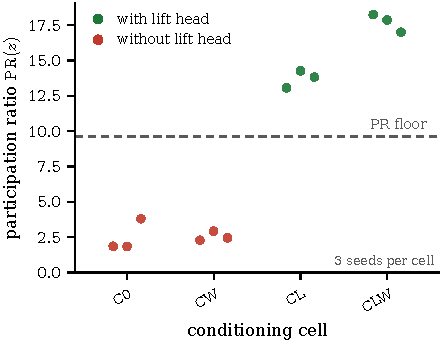
\includegraphics[width=0.92\linewidth]{sections/figures/results/fig_cube_health_v4.pdf}
  \caption{The conditioning cube on the lift and wake axes (\TestSplit{} set,
  three encoder seeds per cell). Left: final participation ratio per cell against
  the collapse floor $0.3\,d = 9.6$, every no-$L$ predictive cell (C0, CW)
  collapsing and every $L$ cell (CL, CLW) healthy. Right: the collapse is flat
  from the start of training while a healthy cell crosses the floor within the
  first quarter of the run. The near-body ($N$) cells and the paired peak-load
  increments are in appendix~\ref{app:nearbody}.}
  \label{fig:cube}
\end{figure}

